\documentclass[aspectratio=169]{beamer}
\usetheme{metropolis}

%\usepackage{beamerthemesplit}
%\beamertemplatenavigationsymbolsempty
\usepackage{amsmath}
\usepackage{amsthm}
\usepackage{amssymb}
\usepackage{latexsym}
\usepackage{graphicx}
\usepackage{fancybox}
\usepackage{dsfont}
\usepackage{multirow} 
\usepackage{multicol}
\usepackage{booktabs} 
\usepackage{dcolumn}
\usepackage{soul}
\usepackage[cache=false]{minted}
\usepackage{MnSymbol}
\usepackage{stmaryrd}


\DeclareMathOperator*{\argmax}{arg\,max}
\DeclareMathOperator*{\argmin}{arg\,min}

\newcommand{\X}{\mathtt{X}}
\newcommand{\Y}{\mathtt{Y}}

%\newcommand{\R}{\mathbb{R}}
%\newcommand{\E}{\mathbb{E}}
%\newcommand{\V}{\mathbb{V}}
\newcommand{\p}{\mathbb{P}}
\newcommand*\df{\mathop{}\!\mathrm{d}}
\newcommand{\del}{\partial}


% imports
\usepackage{xargs}
\usepackage{xpatch}
\usepackage{etoolbox}
\usepackage{pdflscape}
\usepackage{booktabs}
\usepackage{threeparttable}
\usepackage[skip=0.2\baselineskip]{caption}

% command for inputting raw latex
\makeatletter
\newcommand\primitiveinput[1]{\@@input #1 }
\makeatother

% common table command
\newcommandx{\tablecontent}[4]{
    \begin{threeparttable}[!ht]
        \centering
        \caption{#3}
        \vspace{-1em}
        \footnotesize
        \begin{tabular}{#1}
            \primitiveinput{../tables/#2.tex}
        \end{tabular}
        \vspace{-0.2em}
        \begin{tablenotes}[flushleft]
            #4
        \end{tablenotes}
    \end{threeparttable}
}




% \usepackage{slashbox}
\title{Lecture 2: Maximum Likelihood and Friends}
\author{Chris Conlon }
\institute{NYU Stern }


\newcommand{\norm}[1]{\left\lVert#1\right\rVert}
\newcommand{\R}{\mathbb{R}}
\newcommand{\E}{\mathbb{E}}
\newcommand{\V}{\mathbb{V}}
\newcommand{\ol}{\overline}
%\newcommand{\ul}{\underline}
\newcommand{\pp}{{\prime \prime}}
\newcommand{\ppp}{{\prime \prime \prime}}
\newcommand{\policy}{\gamma}


\newcommand{\fp}{\frame[plain]}

\date{\today}

\begin{document}
\maketitle

\begin{frame}{Introduction}
Consider a linear regression with $\varepsilon_i | X_i \sim N(0,\sigma^2)$
\begin{align*}
Y_{it} &= X_{i}'\beta_i + \varepsilon_{i}
\end{align*}
We've discussed the \alert{least squares estimator}:
\begin{align*}
\widehat{\beta}_{ols} &= \arg \min_{\beta} \sum_{i=1}^N (Y_i - X_i' \beta)^2\\
\widehat{\beta}_{ols} &= (\mathbf{X}'\mathbf{X})^{-1} \mathbf{X}' \mathbf{Y}
\end{align*}
\end{frame}


\begin{frame}{Review: What is a Likelihood?}
Suppose we write down the joint distribution of our data $(y_i,x_i)$ for $i=1,\ldots,n$.
\begin{align*}
Pr(y_1,\ldots,y_n, x_1,\ldots,x_n | \theta)
\end{align*}
If  $(y_i,x_i)$ are I.I.D then we can write this as:
\begin{align*}
 Pr(y_1,\ldots,y_n, x_1,\ldots,x_n | \theta) = \prod_{i=1}^N Pr(y_i, x_i | \theta) \propto \prod_{i=1}^N Pr(y_i | x_i , \theta)=L( \mathbf{y}| \mathbf{x} ,\theta )
\end{align*}
We call this $L( \mathbf{y}| \mathbf{x} ,\theta )$ the \alert{likelihood} of the observed data.
\end{frame}




\begin{frame}{MLE: Example}
If we know the distribution of $\varepsilon_i$ we can construct a \alert{maximum likelihood estimator}
\begin{align*}
(\widehat{\beta}_{MLE},\widehat{\sigma}^2_{MLE}) &= \arg \min_{\beta,\sigma^2} L(\beta,\sigma^2)
\end{align*}
Where 
\begin{align*} 
L(\beta,\sigma^2) &= \prod_{i=1}^N p(y_i | x_i,\beta,\sigma^2) \\
                  &= \prod_{i=1}^N \frac{1}{\sqrt{2 \pi \sigma^2}} \exp \left[-\frac{1}{2\sigma^2}(Y_i - X_i' \beta)^2 \right]\\
\ell(\beta,\sigma^2) &= \sum_{i=1}^N -\frac{1}{2} \ln (2 \pi \sigma^2) - \frac{1}{2 \sigma^2} \sum_{i=1}^N(Y_i - X_i' \beta)^2
\end{align*}
\end{frame}

\begin{frame}{MLE: FOC's}
Take the FOC's
\begin{align*}
\ell(\beta,\sigma^2) &= -\frac{N}{2} \ln (2 \pi \sigma^2) - \frac{1}{2 \sigma^2} \sum_{i=1}^N(Y_i - X_i' \beta)^2
\end{align*}
Where 
\begin{align*} 
\frac{ \partial \ell(\beta,\sigma^2) }{\partial \beta}&= \frac{1}{ \sigma^2}\sum_{i=1}^N(Y_i - X_i' \beta) = 0 \rightarrow \widehat{\beta}_{MLE}= \widehat{\beta}_{OLS}\\ 
\frac{ \partial \ell(\beta,\sigma^2) }{\partial \sigma^2}&= -N \frac{1}{2 \sigma^2}  -  \frac{1}{2 \sigma^4} \sum_{i=1}^N(Y_i - X_i' \beta)^2 = 0 \\
\sigma^2_{MLE} &= \frac{1}{N} \sum_{i=1}^N (Y_i - X_i' \beta)^2
\end{align*}
Note: the unbiased estimator uses $\frac{1}{N-K-1}$.
\end{frame}

\begin{frame}{MLE: General Case}
\begin{enumerate}
\item Start with the \alert{joint density of the data} $Z_1,\ldots,Z_N$ with density $f_Z(z,\theta)$
\item Construct the likelhood function of the sample $z_1,\ldots,z_n$
\begin{align*}
L(\mathbf{z} | \theta) = \prod_{i=1}^N f_Z(z_i,\theta)
\end{align*}
\item Construct the \alert{log likelihood} (this has the same $\arg \max$)
\begin{align*}
\ell(\mathbf{z} | \theta) = \sum_{i=1}^N \ln f_Z(z_i,\theta)
\end{align*}
\item Take the FOC's to find $\widehat{\theta}_{MLE}$
\begin{align*}
\theta : \frac{\partial \ell(\theta)}{\partial \theta} =0
\end{align*}
\end{enumerate}
\end{frame}

\begin{frame}{MLE in Detail}
Basic Setup: we know $F(z|\theta_0)$ but not $\theta_0$. We know $\theta_0 \in \Theta \subset \mathbb{R}^K$.
\begin{itemize}
\item Begin with a sample of $z_i$ from $i=1,\ldots,N$ which are I.I.D. with CDF $F(z|\theta_0)$.
\item The MLE chooses
\begin{align*}
\widehat{\theta}_{MLE} = \arg \max_{\theta} \ell(\theta) = \arg \max_{\theta} \sum_{i=1}^N \ln f_Z(z_i,\theta)
\end{align*}
\end{itemize}
\end{frame}


\begin{frame}{MLE: Technical Details}
\begin{enumerate}
\item Consistency. When is it true that for $\epsilon>0$?
\begin{align*}
\lim _ { N \rightarrow \infty } \operatorname { Pr } \left( \left\| \hat { \theta } _ { m l e } - \theta _ { 0 } \right\| > \varepsilon \right) = 0
\end{align*}
\item Asymptotic Normality. What else do we need to show?
\begin{align*}
\sqrt { N } \left( \hat { \theta } _ { m l e } - \theta _ { 0 } \right) \stackrel { d } { \longrightarrow } \mathcal { N } \left( 0 , - \left[ E \frac { \partial ^ { 2 } } { \partial \theta \partial \theta ^ { \prime } } \left( Z _ { i } , \theta _ { 0 } \right) \right] ^ { - 1 } \right)
\end{align*}
\item Optimization. How to we obtain $\widehat{\theta}_{MLE}$ anyway?
\end{enumerate}
\end{frame}


\begin{frame}{MLE: Example \# 1}
\begin{itemize}
\item $Z_i \sim N(\theta_0,1)$ and $\Theta = (-\infty,\infty)$. In this case:
\begin{align*}
\ell ( \theta ) = - N \cdot \ln ( 2 \pi ) - \sum _ { i = 1 } ^ { N } \left( z _ { i } - \theta \right) ^ { 2 } / 2
\end{align*}
\item MLE is $\widehat{\theta}_{MLE}=\overline{z}$ which is consistent for $\theta_0 = E[Z_i]$
\item Asymptotic distribution is $\sqrt{N} ( \overline{z}-\theta_0) \sim N(0,1)$.
\item Calculating mean is easy!
\end{itemize}
\end{frame}




\begin{frame}{MLE: Example \# 2}
\begin{itemize}
\item $Z_i = (Y_i, X_i)$---   $X_i$ has finite mean and variance (but arbitrary distribution)
\item $(Y_i | X_i  =x) \sim N(x' \beta_0, \sigma_0^2)$
\begin{align*}
\widehat{\beta}_{MLE} &= (X'X)^{-1} X'Y\\
\widehat{\sigma}^2_{MLE} &= \frac{1}{N} \sum (y_i - x_i \widehat{\beta}_{MLE})^2
\end{align*}
\item We already have shown consistency and AN for linear regression with normally distributed errors...
\end{itemize}
\end{frame}


\begin{frame}{MLE: Example \# 3}
\begin{itemize}
\item $Z_i = (Y_i, X_i)$---   $X_i$ has finite mean and variance (but arbitrary distribution)
\item $Pr(Y_i=1 | X_i =x) =  \frac{e^{x' \theta_0}}{1+ e^{x'\theta_0}}$
\item Solution is the \alert{logit} model.
\item No simple MLE solution, establishing properties is not obvious...
\end{itemize}
\end{frame}

\begin{frame}{Jensen's Inequality}
Let $g(z)$ be a convex function. Then $\mathbb { E }[g(Z)] \geq g(\mathbb { E }[Z])$, with equality only in the case of a linear function.
\end{frame}

\begin{frame}{More Technical Details}
Define $Y$ as the ratio of the density at $\theta$ to the density at the true value $\theta_0$ both evaluated at $Z$
\begin{align*}
Y = \frac{f_Z(Z;\theta)}{f_Z(Z;\theta_0)}
\end{align*}
\begin{itemize}
\item Let $g(a) = -\ln(a)$ so that $g'(a) = \frac{-1}{a}$ and $g''(a) =\frac{1}{a^2}$.
\item Then by \alert{Jensen's Inequality} $\mathbb{E}[- \ln Y] \geq - \ln \mathbb{E}[Y]$.
\item This gives us
\begin{align*}
\mathbb { E }_z \left[ - \ln \left( \frac { f _ { Z } ( Z ; \theta ) } { f _ { Z } \left( Z ; \theta _ { 0 } \right) } \right) \right] \geq - \ln \left( \mathbb { E }_z \left[ \frac { f _ { Z } ( Z ; \theta ) } { f _ { Z } \left( Z ; \theta _ { 0 } \right) } \right] \right)
\end{align*}
\item The RHS is
\begin{align*}
\mathbb { E }_z \left[ \frac { f _ { Z } ( Z ; \theta ) } { f _ { Z } \left( Z ; \theta _ { 0 } \right) } \right] = \int \frac { f _ { Z } ( z ; \theta ) } { f _ { Z } \left( z ; \theta _ { 0 } \right) } \cdot f _ { Z } \left( z ; \theta _ { 0 } \right) d z = \int f _ { Z } ( z ; \theta ) d z = 1
\end{align*}
\end{itemize}
\end{frame}


\begin{frame}{More Technical Details}
Because $\log(1)=0$ this implies:
\begin{align*}
\mathbb { E }_z \left[ - \ln \left( \frac { f _ { Z } ( Z ; \theta ) } { f _ { Z } \left( Z ; \theta _ { 0 } \right) } \right) \right] \geq 0
\end{align*}
Therefore 
\begin{align*}
- \mathbb { E } \left[ \ln f _ { Z } ( Z ; \theta ) \right] &+ \mathbb { E } \left[ \ln f _ { Z } \left( Z ; \theta _ { 0 } \right) \right] \geq 0\\
\mathbb { E } \left[ \ln f _ { Z } \left( Z ; \theta _ { 0 } \right) \right] &\geq \mathbb { E } \left[ \ln f _ { Z } ( Z ; \theta ) \right]
\end{align*}
\begin{itemize}
\item We maximize the expected value of the log likelihood at the true value of $\theta$!
\item Helpful to work with $\mathbb{E}[\log f(z; \theta)]$ sometimes.
\end{itemize}
\end{frame}


\begin{frame}{Information Matrix Equality}
We can relate the \alert{Fisher Information} to the Hessian of the log-likelihood
\begin{align*}
\mathcal { I } \left( \theta _ { 0 } \right) = - \mathbb { E } \left[ \frac { \partial ^ { 2 } \ln f } { \partial \theta \partial \theta } \left( z ; \theta _ { 0 } \right) \right] 
= \mathbb { E } \left[ \frac { \partial \ln f } { \partial \theta } \left( z ; \theta _ { 0 } \right) \times \frac { \partial \ln f } { \partial \theta  } \left( z ; \theta _ { 0 } \right)' \right]
\end{align*}
\begin{itemize}
    \item This is sometimes known as the \alert{outer product of scores}.
    \item This matrix is \alert{negative definite}
    \item Recall that $ \mathbb { E } \left[ \frac { \partial \ln f } { \partial \theta } \left( z ; \theta _ { 0 } \right) \right]\approx 0$ at the maximum
\end{itemize}
\end{frame}


\begin{frame}{Proof}
\begin{align*}
1 = \int _ { z } f _ { Z } ( z ; \theta ) d z \Rightarrow 0 = \frac { \partial } { \partial \theta } \int _ { z } f _ { Z } ( z ; \theta ) d z
\end{align*}
With some regularity conditions
\begin{align*}
0 = \int _ { z } \frac { \partial f _ { Z } } { \partial \theta } ( z ; \theta ) d z = \underbrace{\int _ { z } \frac { \partial \ln f _ { Z } } { \partial \theta } ( z ; \theta ) \cdot f _ { Z } ( z ; \theta ) d z}_{\mathbb { E } \left[ \frac { \partial \ln f _ { Z } } { \partial \theta } \left( z ; \theta _ { 0 } \right) \right]}
\end{align*}

\begin{itemize}
    \item This gives us the FOC we needed.
    \item Can get information identity with another set of derivatives.
    \end{itemize}
\end{frame}


\begin{frame}{The Cramer-Rao Bound}
We can relate the \alert{Fisher Information} to the Hessian of the log-likelihood
\begin{align*}
\mathcal { I } ( \theta ) = - \mathbb { E } \left[ \frac { \partial ^ { 2 } \ln f } { \partial \theta \partial \theta ^ { \prime } } ( Z | \theta ) \right]
\end{align*}
It turns out this provides a bound on the variance
\begin{align*}
\operatorname { Var } ( \hat { \theta } ( Z ) ) \geq \mathcal { I } \left( \theta _ { 0 } \right) ^ { - 1 }
\end{align*}
Because we can't do better than Fisher Information we know that MLE is most efficient estimator!
\end{frame}

\begin{frame}{MLE: Discussion}
Tradeoffs
\begin{itemize}
\item How does this compare to GM Theorem?
\item If MLE is most efficient estimate, why ever use something else?
\end{itemize}
\end{frame}


\begin{frame}{Exponential Example}
\begin{align*}
f _ { Y | X } ( y | x , \beta _ { 0 } ) =  { e } ^ { x ^ { \prime } \beta _ { 0 } } \exp \left( - y  { e } ^ { x ^ { \prime } \beta _ { 0 } } \right)
\end{align*}
With log likelihood
\begin{align*}
\ell( \beta ) = \sum _ { i = 1 } ^ { N } \ln f _ { Y | X } \left( y _ { i } | x _ { i } , \beta \right) = \sum _ { i = 1 } ^ { N } X _ { i } ^ { \prime } \beta - y _ { i } \cdot \exp \left( x _ { i } ^ { \prime } \beta \right)
\end{align*}
And Score, Hessian, and Information Matrix:
\begin{align*}
\mathcal { S }_i ( y_i, x_i , \beta ) &= x_i ^ { \prime } \left( 1 - y_i \exp \left( x_i ^ { \prime } \beta \right) \right)\\
\mathcal { H }_i ( y_i , x_i , \beta ) &= - y_i x_i x_i ^ { \prime } \exp \left( x_i ^ { \prime } \beta \right)\\
% WHERE DOES THIS COME FROM
\mathcal { I } \left( \beta _ { 0 } \right) &= \mathbb { E } \left[ Y X X ^ { \prime } \exp \left( X ^ { \prime } \beta _ { 0 } \right) \right] = \mathbb { E } \left[ X X ^ { \prime } \right]
\end{align*}
\end{frame}


\section*{Computing Maximum Likelihood Estimators}

\begin{frame}{Newton's Method for Root Finding}
Consider the Taylor series for $f(x)$ approximated around $f(x_0)$:
\begin{align*}
f(x) \approx f(x_0) + f'(x_0) \cdot (x-x_0) + f''(x_0) \cdot (x-x_0)^2 + o_p(3)
\end{align*}
Suppose we wanted to find a \alert{root} of the equation where $f(x^{*})=0$ and solve for $x$:
\begin{align*}
0 &= f(x_0) + f'(x_0) \cdot (x-x_0) \\
x_1 &= x_0-\frac{f(x_0)}{f'(x_0)} 
\end{align*}
This gives us an \alert{iterative} scheme to find $x^{*}$:
\begin{enumerate}
\item Start with some $x_k$. Calculate $f(x_k),f'(x_k)$
\item Update using $x_{k+1} = x_k - \frac{f(x_k)}{f'(x_k)} $
\item Stop when $|x_{k+1}-x_{k}| < \epsilon_{tol}$.
\end{enumerate}
\end{frame}

\begin{frame}{Newton-Raphson for Minimization}
We can re-write \alert{optimization} as \alert{root finding};
\begin{itemize}
\item We want to know $\hat{\theta} = \arg \max_{\theta} \ell(\theta)$.
\item Construct the FOCs $\frac{\partial \ell}{\partial \theta}=0 \rightarrow$  and find the zeros.
\item How? using Newton's method! Set $f(\theta) = \frac{\partial \ell}{\partial \theta}$
\end{itemize}
\begin{align*}
\theta_{k+1} &= \theta_k -  \left[ \frac{\partial^2 \ell}{\partial \theta^2}(\theta_k) \right]^{-1} \cdot \frac{\partial \ell}{\partial \theta}(\theta_k)
\end{align*}
The SOC is that $ \frac{\partial^2 \ell}{\partial \theta^2} >0$. Ideally at all $\theta_k$.\\
This is all for a \alert{single variable} but the \alert{multivariate} version is basically the same.
\end{frame}


\begin{frame}{Newton's Method: Multivariate}
Start with the objective $Q(\theta) = - \ell(\theta)$:
\begin{itemize}
\item Approximate $Q(\theta)$ around some initial guess $\theta_0$ with a quadratic function
\item Minimize the quadratic function (because that is easy) call that $\theta_1$
\item Update the approximation and repeat.
\begin{align*}
\theta_{k+1} = \theta_k - \left[ \frac{\partial^2 Q}{\partial \theta \partial \theta'} \right]^{-1}\frac{\partial Q}{\partial \theta}(\theta_k)
\end{align*}
\item The equivalent SOC is that the {Hessian Matrix} is \alert{positive semi-definite}  (ideally at all $\theta$).
\item In that case the problem is \alert{globally convex} and has a \alert{unique maximum} that is easy to find.
\end{itemize}
\end{frame}


\begin{frame}{Newton's Method}
We can generalize to Quasi-Newton methods:
\begin{align*}
\theta_{k+1} = \theta_k -  \lambda_k \underbrace{\left[ \frac{\partial^2 Q}{\partial \theta \partial \theta'} \right]^{-1}}_{A_k} \frac{\partial Q}{\partial \theta}(\theta_k)
\end{align*}
Two Choices:
\begin{itemize}
\item Step length $\lambda_k$
\item Step direction $d_k=A_k \frac{\partial Q}{\partial \theta}(\theta_k)$
\item Often rescale the direction to be unit length $\frac{d_k}{\norm{d_k}}$.
\item If we use $A_k$ as the true Hessian and $\lambda_k=1$ this is a \alert{full Newton step}.
\end{itemize}
\end{frame}

\begin{frame}{Newton's Method: Alternatives}
Choices for $A_k$
\begin{itemize}
\item $A_k= I_{k}$ (Identity) is known as \alert{gradient descent} or \alert{steepest descent}
\item BHHH. Specific to MLE. Exploits the \alert{Fisher Information}.
\begin{align*}
A _ { k } 
&= \left[ \frac { 1 } { N } \sum _ { i = 1 } ^ { N } \frac { \partial \ln f } { \partial \theta } \left( \theta _ { k } \right) \frac { \partial \ln f } { \partial \theta ^ { \prime } } \left( \theta _ { k } \right) \right] ^ { - 1 }\\
&=- \mathbb { E } \left[ \frac { \partial ^ { 2 } \ln f } { \partial \theta \partial \theta ^ { \prime } } \left( Z , \theta ^ { * } \right) \right] 
= \mathbb { E } \left[ \frac { \partial \ln f } { \partial \theta } \left( Z , \theta ^ { * } \right) \frac { \partial \ln f } { \partial \theta ^ { \prime } } \left( Z , \theta ^ { * } \right) \right]
\end{align*}
\item Alternatives \alert{SR1} and \alert{DFP} rely on an initial estimate of the Hessian matrix and then approximate an update to $A_k$.
\item Usually updating the Hessian is the costly step.
\item Non invertible Hessians are bad news.
\end{itemize}
\end{frame}

\section{Extended Example: Binary Choice}
\begin{frame}
\frametitle{Binary Choice: Overview}
Many problems we are interested in look at discrete rather than continuous outcomes:
\begin{itemize}
\item Entering a Market/Opening a Store
\item Working or a not
\item Being married or not
\item Exporting to another country or not
\item Going to college or not
\item Smoking or not
\item etc.
\end{itemize}
\end{frame}

\begin{frame}
\frametitle{Simplest Example: Flipping a Coin}
Suppose we flip a coin which is yields heads ($Y=1$) and tails ($Y=0$). We want to estimate the probability $p$ of heads:
\begin{eqnarray*}
Y_i =
\begin{cases}
1 \mbox{ with probability } p \\
0 \mbox{ with probability } 1-p
\end{cases}
\end{eqnarray*}
We see some data $Y_1,\ldots,Y_N$ which are (i.i.d.)\\
\vspace{0.2cm}
We know that $Y_i \sim Bernoulli(p)$.
\end{frame}


\begin{frame}{Simplest Example: Flipping a Coin}
We can write the likelihood of $N$ Bernoulli trials as 
$$Pr(Y_1 = y_1, Y_2=y_2,\ldots,Y _N=y_N )  =  f(y_1,y_2,\ldots,y_N | p ) $$
\begin{eqnarray*}
&=& \prod_{i=1}^N p^{y_i} (1-p)^{1-y_i}\\
&=& p^{\sum_{i=1}^N y_i} (1-p)^{N-\sum{i=1}^N y_i}
\end{eqnarray*}
And then take logs to get the \alert{log likelihood}:
\begin{eqnarray*}
\ln  f(y_1,y_2,\ldots,y_N | p )  &=& \left( \sum_{i=1}^N y_i \right)  \ln p  + \left(N-\sum_{i=1}^N y_i \right)  (1-p)
\end{eqnarray*}
\end{frame}

\begin{frame}{Simplest Example: Flipping a Coin}
Differentiate the log-likelihood to find the maximum:
\begin{eqnarray*}
\ln  f(y_1,y_2,\ldots,y_N | p )  &=& \left( \sum_{i=1}^N y_i \right)  \ln p  + \left(N-\sum_{i=1}^N y_i \right)  \ln(1-p)\\
\rightarrow 0&=& \frac{1}{\hat{p}}  \left( \sum_{i=1}^N y_i \right) + \frac{-1}{1-\hat{p}}   \left(N-\sum_{i=1}^N y_i \right) \\
 \frac{\hat{p}}{1-\hat{p}} &=& \frac{\sum_{i=1}^N y_i }{N- \sum_{i=1}^N y_i } = \frac{\overline{Y}}{1-\overline{Y}} \\
\hat{p}^{MLE} &=& \overline{Y}
\end{eqnarray*}
That was a lot of work to get the obvious answer: \alert{fraction of heads}.
\end{frame}

\begin{frame}{More Complicated Example: Adding Covariates}
We probably are interested in more complicated cases where $p$ is not the same for all observations but rather $p(X)$ depends on some covariates. Here is an example from the Boston HMDA Dataset:
\begin{itemize}
\item 2380 observations from 1990 in the greater Boston area.
\item Data on: individual Characteristics, Property Characteristics, Loan Denial/Acceptance (1/0).
\item Mortgage Application process circa 1990-1991:
\begin{itemize}
\item Go to bank
\item Fill out an application (personal+financial info)
\item Meet with loan officer
\item Loan officer makes decision
\begin{itemize}
\item Legally in race blind way (discrimination is illegal but rampant)
\item Wants to maximize profits (ie: loan to people who don't end up defeaulting!)
\end{itemize}
\end{itemize}
\end{itemize}
\end{frame}


\begin{frame}{Loan Officer's Decision}
Financial Variables:
\begin{itemize}
\item $P/I$ ratio
\item housing expense to income ratio
\item loan-to-value ratio
\item personal credit history (FICO score, etc.)
\item Probably some nonlinearity:
\begin{itemize}
\item Very high $LTV > 80\%$ or $>95\%$ is a bad sign (strategic defaults?)
\item Credit Score Thresholds
\end{itemize}
\end{itemize}
\end{frame}


\begin{frame}{Loan Officer's Decision}
Goal $Pr(Deny=1 | black, X)$\\

\begin{itemize}
\item Lots of potential \alert{omitted variables} which are correlated with race
\begin{itemize}
\item Wealth, type of employment
\item family status
\item credit history
\item zip code of property
\end{itemize}
\item Lots or \alert{redlining} cases hinge on whether or not black applicants were treated in a discriminatory way.
\end{itemize}
\end{frame}

\begin{frame}
\begin{center}
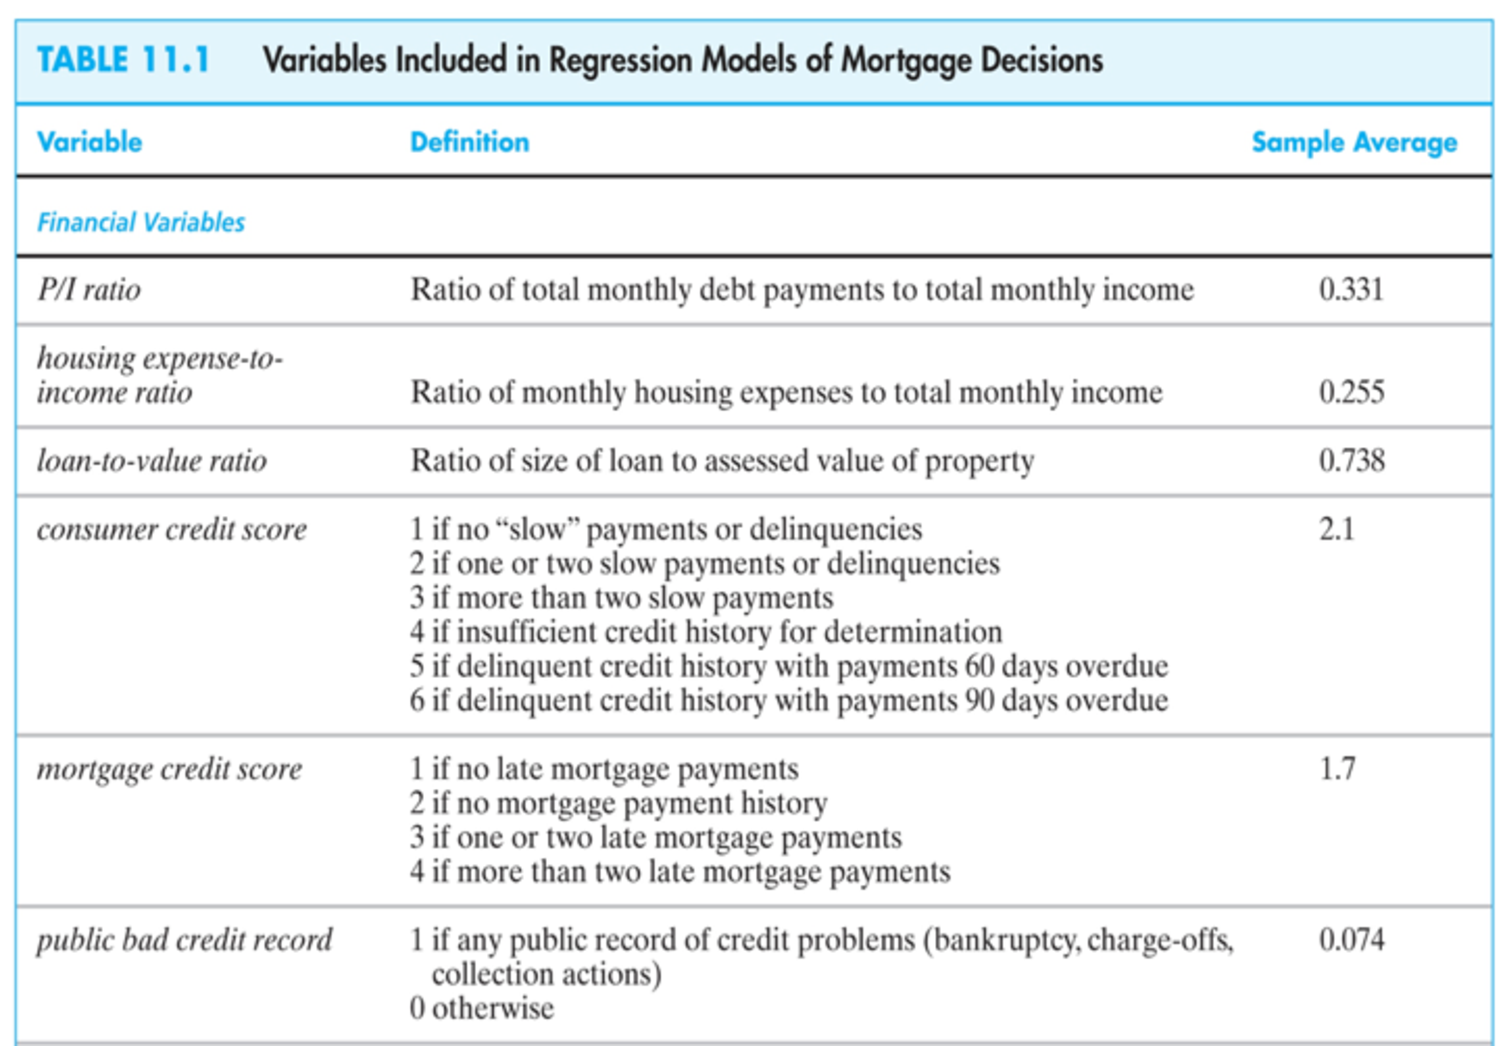
\includegraphics[width=3.25in]{resources/hmda1.pdf}\\
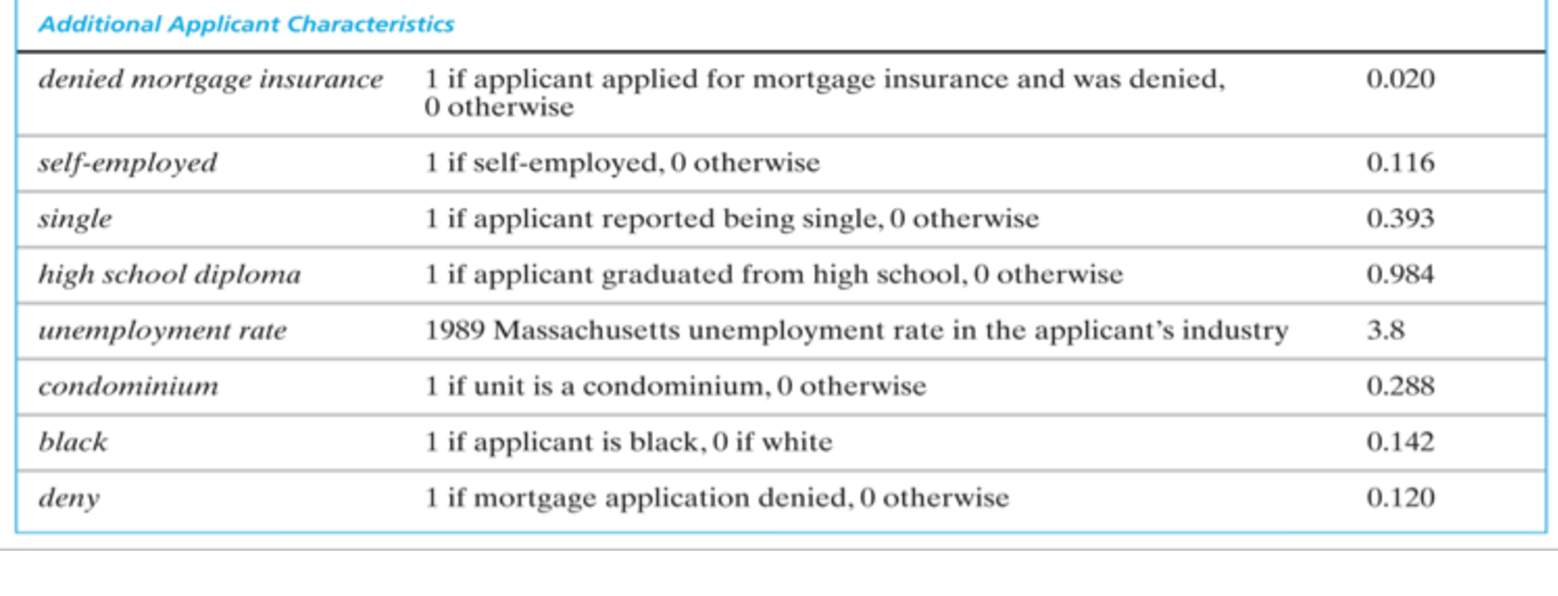
\includegraphics[width=3.25in]{resources/hmda2.pdf}
\end{center}
\end{frame}


\begin{frame}{Linear Probability Model}
First thing we might try is OLS
\begin{eqnarray*}
Y_i  = \beta_0 + \beta_1 X_i + \varepsilon_i
\end{eqnarray*}
\begin{itemize}
\item What does $\beta_1$ mean when $Y$ is binary? Is $\beta_1  = \frac{\Delta Y}{\Delta X}$?
\item What does the line $\beta_0 + \beta_1 X$ when $Y$ is binary?
\item What does the predicted value $\hat{Y}$ mean when $Y$ is binary? Does $\hat{Y} = 0.26$ mean that someone gets approved or denied for a loan?
\end{itemize}
\end{frame}

\begin{frame}{Linear Probability Model}
OLS is called the \alert{linear probability model} 
\begin{eqnarray*}
Y_i  = \beta_0 + \beta_1 X_i + \varepsilon_i 
\end{eqnarray*}
because:
\begin{eqnarray*}
E[Y | X] &=& 1 \times Pr(Y=1 | X) + 0 \times Pr(Y=0  | X) \\
Pr(Y=1 | X) &=& \beta_0 + \beta_1 X_i + \varepsilon_i
\end{eqnarray*}
The predicted value is a \alert{probability} and 
\begin{eqnarray*}
\beta_1 = \frac{Pr(Y=1 | X =x+\Delta x) - Pr(Y=1 | X=x)}{\Delta x}
\end{eqnarray*}
So $\beta_1$ represents the average change in probability that $Y=1$ for a unit change in $X$.
\end{frame}


\begin{frame}
\begin{center}
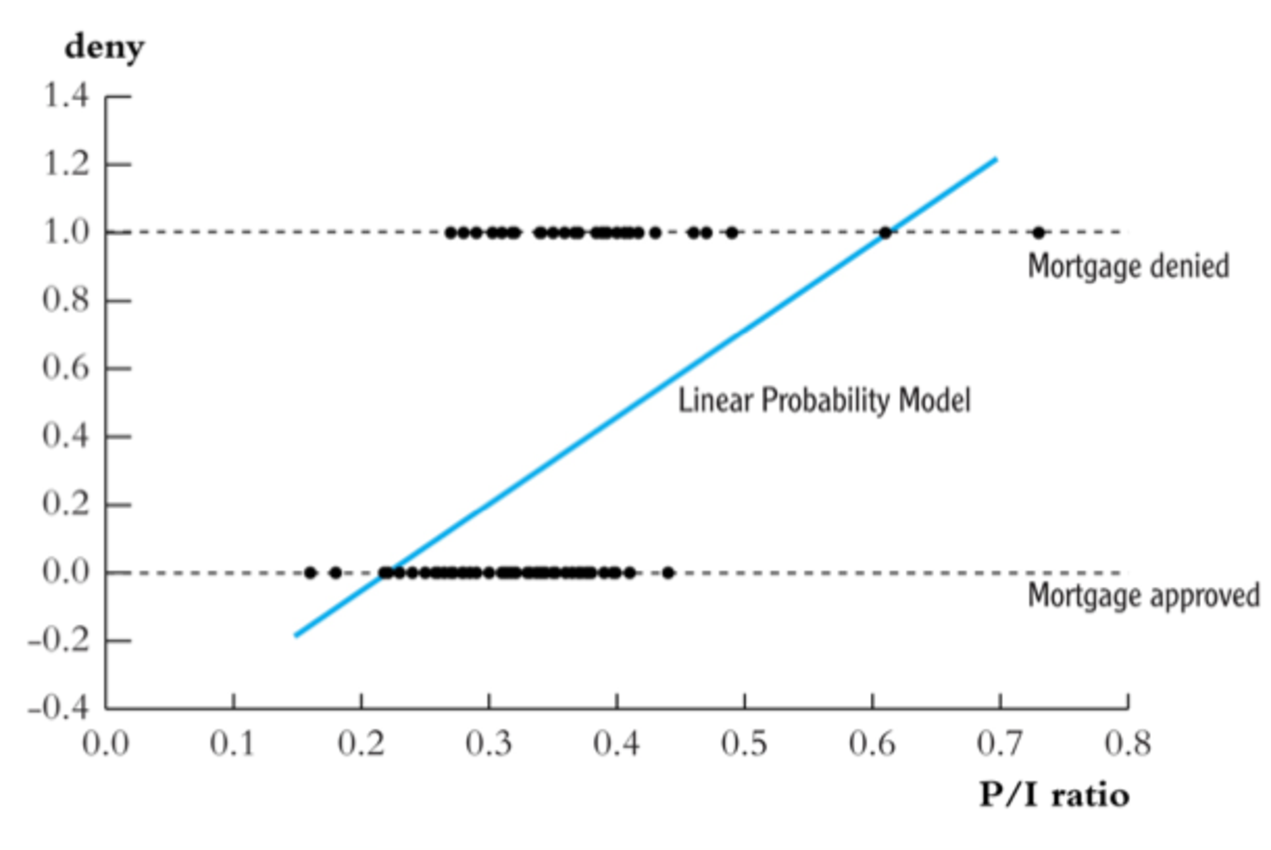
\includegraphics[width=5in]{resources/lpm.pdf}\\
\end{center}
\end{frame}

\begin{frame}{That didn't look great}
\begin{itemize}
\item Is the marginal effect $\beta_1$ actually constant or does it depend on $X$?
\item Sometimes we predict $\hat{Y} >1$ or $\hat{Y} <0$. What does that even mean? Is it still a probability?
\item Fit in the middle seems not so great -- what does $\hat{Y} = 0.5$ mean?
\end{itemize}
\end{frame}

\begin{frame}{Results}
\begin{eqnarray*}
\widehat{deny_i}= -.091& + .559 \cdot \text{P/I ratio} + &.177 \cdot \text{black} \\
(0.32)&( .098) & (.025)\\
\end{eqnarray*}
Marginal Effects: 
\begin{itemize}
\item Increasing $P/I$ from $0.3 \rightarrow 0.4$ increases probabilty of denial by $5.59$ percentage points. (True at all level of $P/I$).
\item At all $P/I$ levels blacks are $17.7$ percentage points more likely to be denied.
\item But still some omitted factors.
\item True effects are likely to be \alert{nonlinear} can we add polynomials in $P/I$? Dummies for different levels? 
\end{itemize}
\end{frame}


\begin{frame}{Moving Away from LPM}
Problem with the LPM/OLS is that it requires that \alert{marginal effects are constant} or that probability can be written as linear function of parameters.
\begin{eqnarray*}
Pr(Y=1 | X) = \beta_0 + \beta_1 X+ \epsilon
\end{eqnarray*}
Some desirable properties:
\begin{itemize}
\item Can we restrict our predictions to $[0,1]$?
\item Can we preserve \alert{monotonicity} so that $Pr(Y=1| X)$ is increasing in $X$ for $\beta_1 >0$?
\item Some other properties (continuity, etc.) \pause
\item Want a function $F(z): (-\infty,\infty) \rightarrow [0,1]$.
\item What function will work?
\end{itemize}
\end{frame}

\begin{frame}
\begin{center}
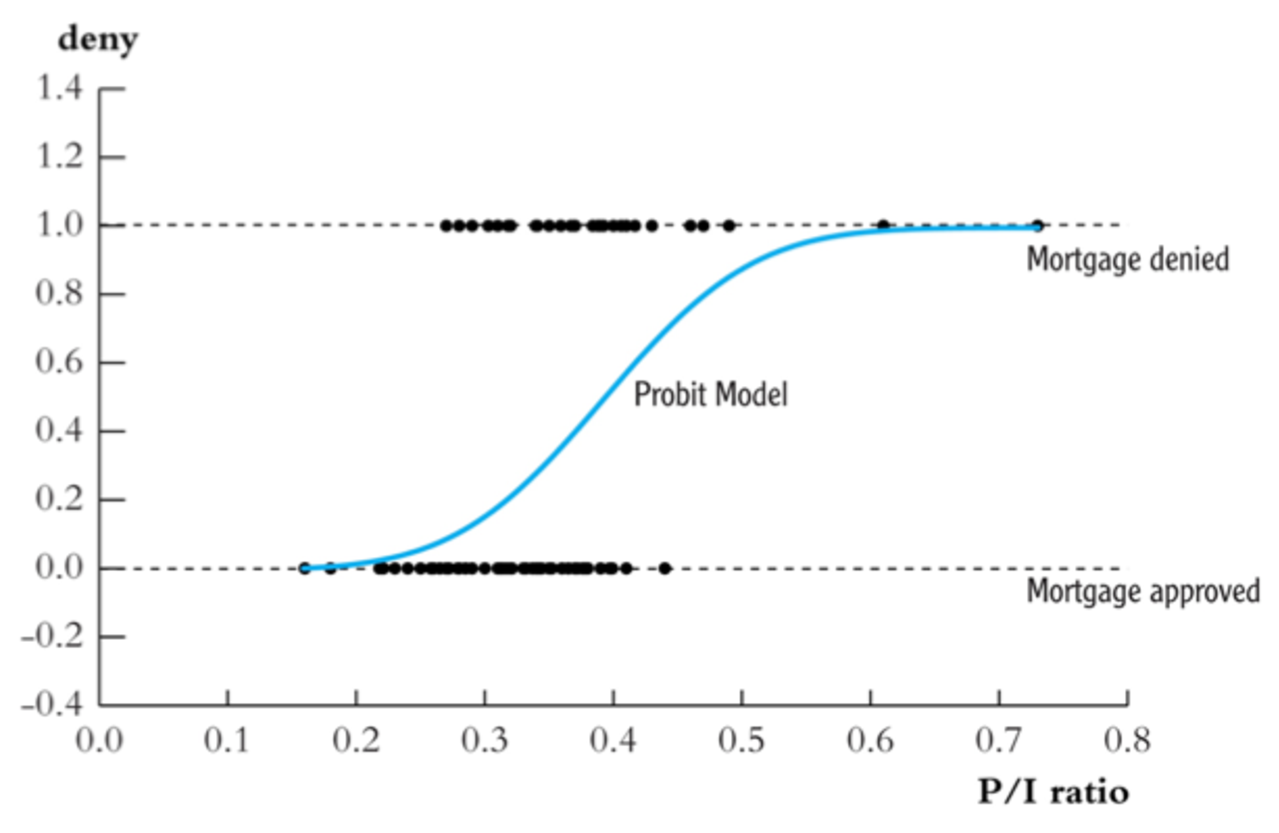
\includegraphics[width=5in]{resources/probit.pdf}
\end{center}
\end{frame}

\begin{frame}{Choosing a transformation}
\begin{eqnarray*}
Pr(Y=1 | X) = F(\beta_0 + \beta_1 X)
\end{eqnarray*}
\begin{itemize}
\item One $F(\cdot)$ that works is $\Phi(z)$ the normal CDF. This is the \alert{probit} model.
\begin{itemize}
\item Actually any CDF would work but the normal is convenient.
\end{itemize}
\item One $F(\cdot)$ that works is $\frac{e^z}{1+ e^z}=\frac{1}{1+e^{-z}}$ the logistic function . This is the \alert{logit} model.
\item Both of these give `S'-shaped curves.
\item The LPM is $F(\cdot)$ is the \alert{identity function} (which doesn't satisfy my $[0,1]$ property).
\item This $F(\cdot)$ is often called a \alert{link function}. Why?
\end{itemize}
\end{frame}


\begin{frame}{Why use the normal CDF?}
Has some nice properties:
\begin{itemize}
\item Gives us more of the `S' shape
\item $Pr(Y=1|X)$ is increasing in $X$ if $\beta_1>0$.
\item $Pr(Y=1|X) \in [0,1]$ for all $X$
\item Easy to use -- you can look up or use computer for normal CDF.
\item Relatively straightforward interpretation
\begin{itemize}
\item $Z=\beta_0 + \beta_1 X$ is the $z$-value.
\item $\beta_1$ is the change in the $z$-value for a change in $X_1$.
\end{itemize}
\end{itemize}
\end{frame}

\begin{frame}
\begin{center}
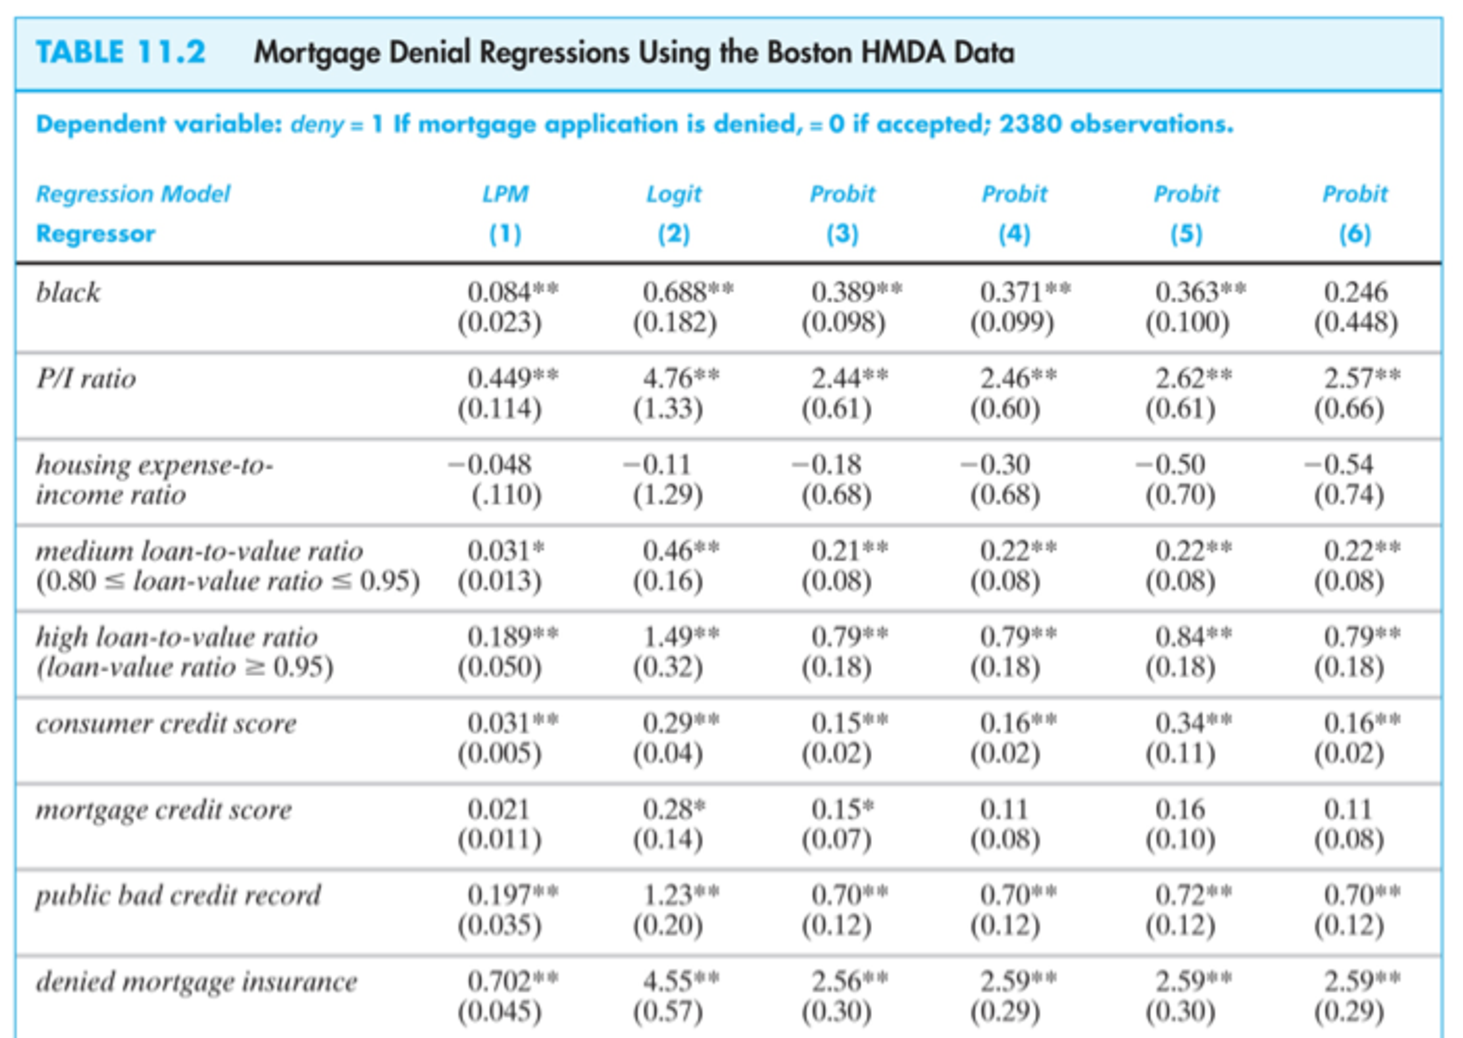
\includegraphics[width=2.5in]{resources/hmda3.pdf}\\
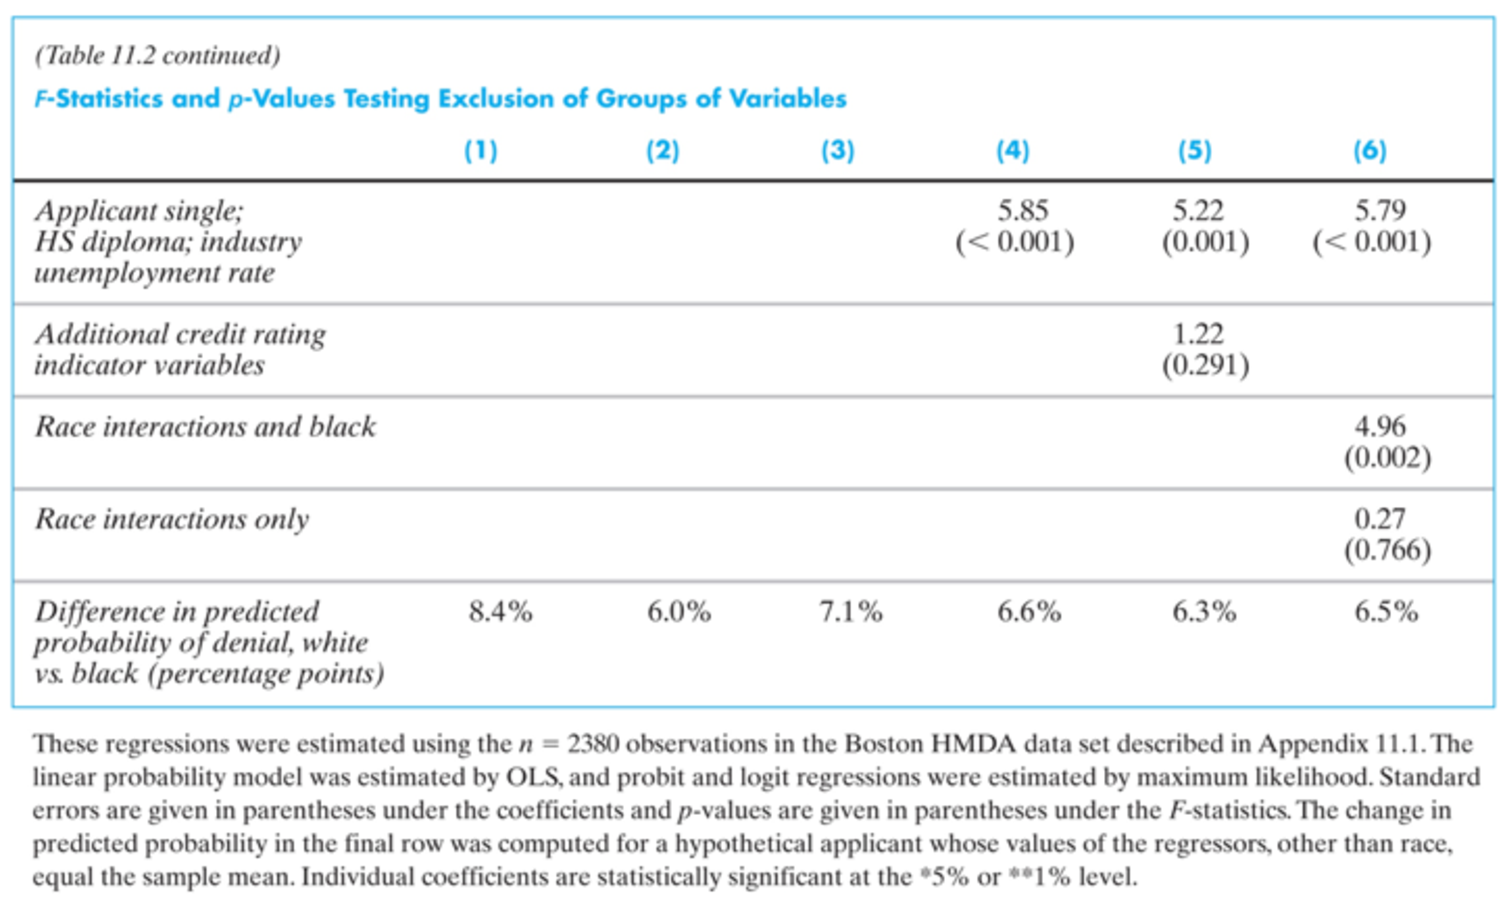
\includegraphics[width=2.5in]{resources/hmda3a.pdf}\\
\end{center}
\end{frame}

\begin{frame}[fragile]{Probit in R}
\footnotesize
\begin{semiverbatim}
bm1 <- glm(deny ~ pi_rat+black, data=hmda, family = binomial(link="probit"))
coeftest(bm1)

z test of coefficients:

             Estimate Std. Error  z value  Pr(>|z|)    
(Intercept) -2.258787   0.136691 -16.5248 < 2.2e-16 ***
pi_rat       2.741779   0.380469   7.2063 5.749e-13 ***
blackTRUE    0.708155   0.083352   8.4959 < 2.2e-16 ***
---
    Signif. codes:  0 `***' 0.001 `**' 0.01 `*' 0.05 `.' 0.1 ` ' 1

predict(bm1, data.frame(pi_rat=.3,black=FALSE),type = "response")
    0.07546516
predict(bm1, data.frame(pi_rat=.3,black=TRUE),type = "response")
    0.2332769
\end{semiverbatim}
\begin{itemize}
\item Probit predicts a 7.5\% chance of mortgage denial for non-black applicants, and 23.3\% chance for black ones.
\end{itemize}
\end{frame}

\begin{frame}{Why use the logistic CDF?}
Has some nice properties:
\begin{itemize}
\item Gives us more of the `S' shape
\item $Pr(Y=1|X)$ is increasing in $X$ if $\beta_1>0$.
\item $Pr(Y=1|X) \in [0,1]$ for all $X$
\item Easy to compute: $\frac{1}{1+e^{-z}}=\frac{e^{z}}{1+e^{z}}$ has analytic derivatives too.
\item Log odds interpretation
\begin{itemize}
\item $\log(\frac{p}{1-p}) = \beta_0 + \beta_1 X$
\item $\beta_1$ tells us how \alert{log odds ratio} responds to $X$.
\item $\frac{p}{1-p} \in (-\infty,\infty)$ which fixes the $[0,1]$ problem in the other direction.
\item more common in other fields (epidemiology, biostats, etc.).
\end{itemize}
\item Also has the property that $F(z) = 1-F(-z)$.
\item Similar to probit but different scale of coefficients
\item Logit/Logistic are sometimes used interchangeably but sometimes mean different things depending on the literature.
\end{itemize}
\end{frame}

\begin{frame}[fragile]{Logit in R}
\footnotesize
\begin{semiverbatim}
bm1 <-glm(deny~pi_rat+black,data=hmda, family=binomial(link="logit"))
coeftest(bm1)

z test of coefficients:

            Estimate Std. Error  z value  Pr(>|z|)    
(Intercept) -4.12556    0.26841 -15.3701 < 2.2e-16 ***
pi_rat       5.37036    0.72831   7.3737  1.66e-13 ***
blackTRUE    1.27278    0.14620   8.7059 < 2.2e-16 ***
---
    Signif. codes:  0 `***' 0.001 `**' 0.01 `*' 0.05 `.' 0.1 ` ' 1

> predict(bm1, data.frame(pi_rat=.3,black=TRUE),type = "response")
0.2241459 
> predict(bm1, data.frame(pi_rat=.3,black=FALSE),type = "response")
0.07485143  
\end{semiverbatim}
\begin{itemize}
\item Logit predicts a 7.5\% chance of mortgage denial for non-black applicants, and 22.4\% chance for black ones. (Very similar to probit).
\end{itemize}
\end{frame}



\begin{frame}
\frametitle{A quick comparison}
\begin{itemize}
\item LPM prediction departs greatly from CDF long before $[0,1]$ limits.
\item We get probabilities that are too extreme even for $X\hat{\beta}$ ``in bounds''.
\item Some (MHE) argue that though $\hat{Y}$ is flawed, constant marginal effects are still OK.
\item Logit and Probit are highly similar
\end{itemize}
\begin{center}
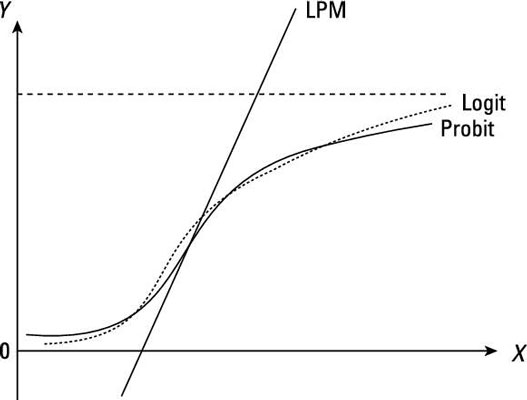
\includegraphics[width=2in]{resources/lpm-probit.jpg}
\end{center}
\end{frame}

\begin{frame}
\begin{center}
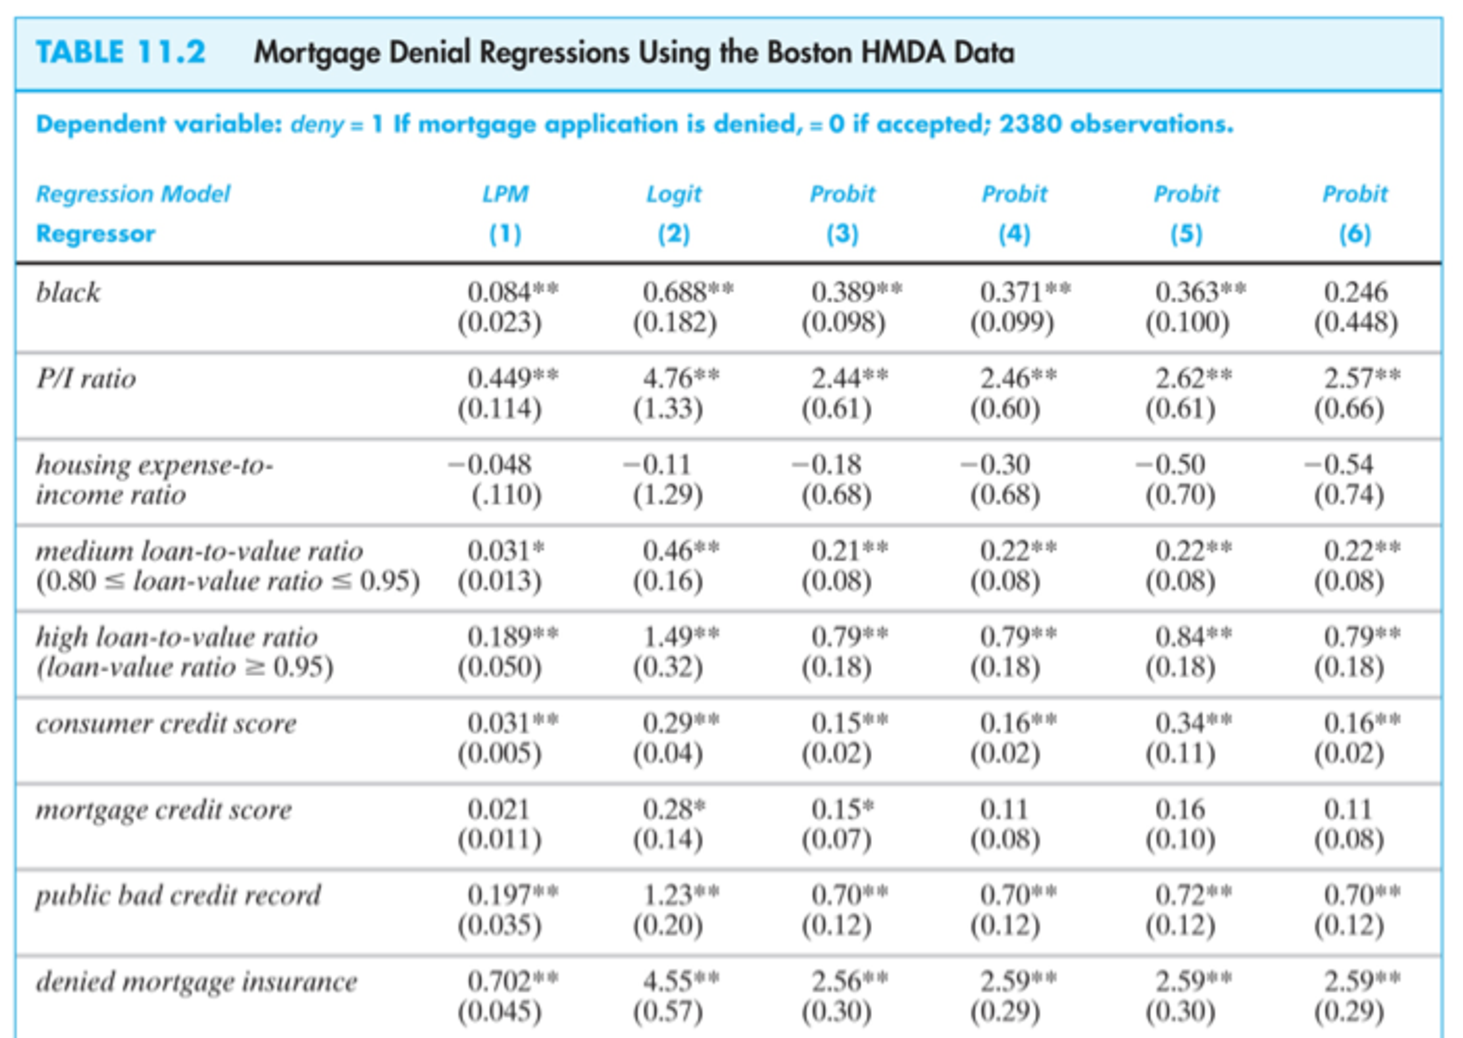
\includegraphics[width=2.5in]{resources/hmda3.pdf}\\
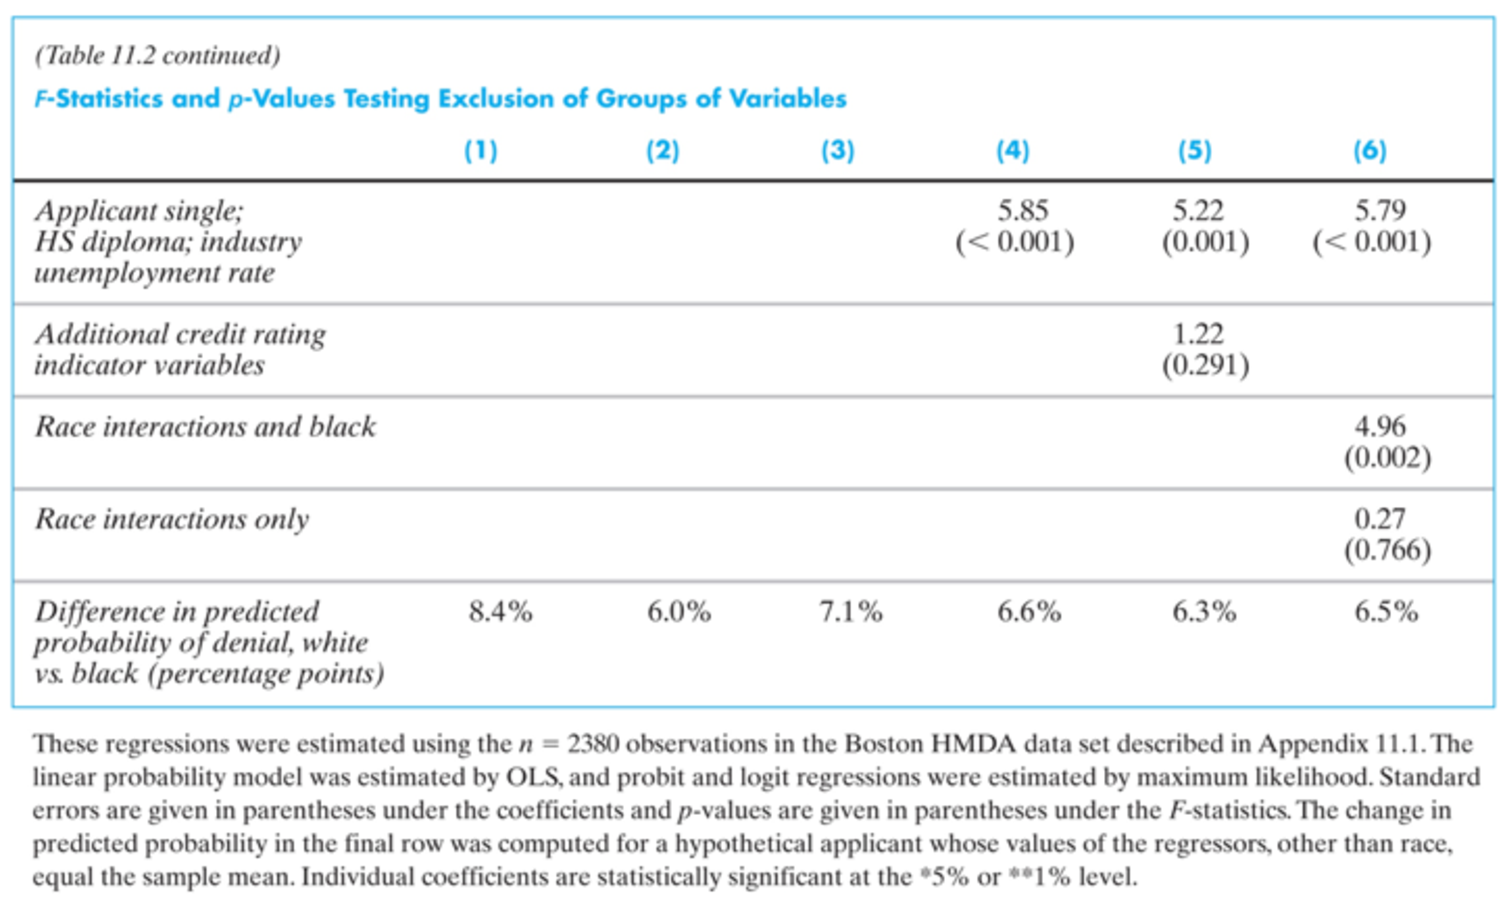
\includegraphics[width=2.5in]{resources/hmda3a.pdf}\\
\end{center}
\end{frame}

\begin{frame}
\frametitle{Latent Variables/ Limited Dependent Variables}
An alternative way to think about this problem is that there is a continuously distributed $Y^{*}$ that we as the econometrician don't observe.
\begin{eqnarray*}
Y_i =
\begin{cases}
1 \mbox{ if } Y^{*} >0 \\
0 \mbox{ if } Y^{*} \leq 0
\end{cases}
\end{eqnarray*}
\begin{itemize}
\item Instead we only see whether $Y^{*}$ exceeds some threshold (in this case $0$).
\item We can think about $Y^{*}$ as a \alert{latent variable}.
\item Sometimes you will see this description in the literature, everything else is the same!
\end{itemize}
\end{frame}


\begin{frame}
\frametitle{Index Models}
We sometimes call these single index models or threshold crossing models
\begin{eqnarray*}
Z_i = X_i \beta
\end{eqnarray*}
\begin{itemize}
\item We start with a potentially large number of regressors in $X_i$ but $X_i \beta = Z_i$ is a \alert{scalar}
\item We can just calculate $F(Z_i)$ for Logit or Probit (or some other CDF).
\item $Z_i$ is the \alert{index}. if $Z_i = X_i \beta$ we say it is a \alert{linear index} model.
\end{itemize}
\end{frame}




\begin{frame}
\frametitle{What does software do?}
\begin{itemize}
\item One temptation might be \alert{nonlinear least squares}:
\begin{eqnarray*}
\hat{\beta}^{NLLS} = \arg \min_{\beta} \sum_{i=1}^N (Y_i - \Phi(X_i \beta))^2
\end{eqnarray*}
\item Turns out this isn't what people do.
\item We can't always directly estimate using the log-odds
\begin{eqnarray*}
\log\left(\frac{p}{1-p}\right)= \beta X_i + \varepsilon_i
\end{eqnarray*}
\item The problem is that $p$ or $p(X_i)$ isn't really observed.
\end{itemize}
\end{frame}

\begin{frame}
\frametitle{What does software do?}
\begin{itemize}
\item Can construct an MLE:
\begin{eqnarray*}
\hat{\beta}^{MLE} &=& \arg \max_{\beta} \prod_{i=1}^N F(Z_i)^{y_i} (1-F(Z_i))^{1-{y_i} }\\
Z_i &=& \beta_0 + \beta_1 X_i
\end{eqnarray*}
\item Probit: $F(Z_i) = \Phi(Z_i)$ and its derivative (density) $f(Z_i) = \phi(Z_i)$. \\
Also is \alert{symmetric} so that $1 - F(Z_i) = F(-Z_i)$.
\item Logit: $F(Z_i) = \frac{1}{1+e^{-z}}$ and its derivative (density) $f(Z_i) = \frac{e^{-z}}{(1+e^{-z})^2}$ a more convenient property is that $\frac{f(z)}{F(z)} = 1 - F(z)$ this is called the \alert{hazard rate}.
\end{itemize}
\end{frame}

\begin{frame}
\frametitle{A probit trick}
Let $q_i = 2 y_i -1$
\begin{eqnarray*}
F(q_i \cdot Z_i) = 
\begin{cases}
F(Z_i)  &\mbox{ when } y_i=1 \\
F(-Z_i) = 1-F(Z_i)& \mbox{ when } y_i=0
\end{cases}
\end{eqnarray*}
So that 
\begin{eqnarray*}
\ell(y_1,\ldots, y_n | \beta) = \sum_{i=1}^N \ln F(q_i \cdot Z_i) 
\end{eqnarray*}
\end{frame}


\begin{frame}
\frametitle{FOC of Log-Likelihood}
\begin{eqnarray*}
\ell(y_1,\ldots,y_n | \beta) &=& \sum_{i=1}^N y_i \ln F(Z_i) + (1-y_i) \ln(1- F(Z_i)) \\
\frac{\partial l }{\partial \beta} &=& \sum_{i=1}^N \frac{y_i}{ F(Z_i)} \frac{ d F}{d \beta}(Z_i) - \frac{1-y_i}{1-F(Z_i)}  \frac{ d F}{d \beta} (Z_i)\\
 &=& \sum_{i=1}^N \frac{y_i \cdot f(Z_i) }{ F(Z_i)} \frac{ d Z_i}{d \beta} -  \sum_{i=1}^N \frac{(1-y_i)\cdot f(Z_i) }{1-F(Z_i)} \frac{ d Z_i}{d \beta} \\
 &=& \sum_{i=1}^N  \left[ \frac{y_i \cdot f(Z_i) }{ F(Z_i)} X_i -  \frac{(1-y_i)\cdot f(Z_i) }{1-F(Z_i)} X_i \right] \\
\end{eqnarray*}
\end{frame}

\begin{frame}
\frametitle{FOC of Log-Likelihood (Logit)}
This is the \alert{score} of the log-likelihood:
\begin{eqnarray*}
\frac{\partial l }{\partial \beta} = \nabla_{\beta} \cdot \ell(\mathbf{y}; \beta) &=&  \sum_{i=1}^N  \left[ y_i \frac{ f(Z_i) }{ F(Z_i)}  -  (1-y_i) \frac{f(Z_i) }{1-F(Z_i)} \right]  \cdot X_i 
\end{eqnarray*}
It is technically also a \alert{moment condition}. It is easy for the logit
\begin{eqnarray*}
 \nabla_{\beta} \cdot \ell(\mathbf{y}; \beta) &=&  \sum_{i=1}^N  \left[ y_i (1-F(Z_i)) -  (1-y_i) F(Z_i) \right] \cdot X_i \\
 &=&  \sum_{i=1}^N  \underbrace{\left[ y_i - F(Z_i) \right]}_{\varepsilon_i} \cdot X_i 
\end{eqnarray*}
This comes from the hazard rate.
\end{frame}

\begin{frame}
\frametitle{FOC of Log-Likelihood (Probit)}
This is the \alert{score} of the log-likelihood:
\begin{eqnarray*}
\frac{\partial l }{\partial \beta} = \nabla_{\beta} \cdot \ell(\mathbf{y}; \beta) &=&  \sum_{i=1}^N  \left[ y_i \frac{ f(Z_i) }{ F(Z_i)}  -  (1-y_i) \frac{f(Z_i) }{1-F(Z_i)} \right] \cdot X_i  \\
 &=&  \sum_{y_i=1}  \frac{\phi(Z_i) }{ \Phi(Z_i)} X_i +\sum_{y_i=0} \frac{-\phi(Z_i) }{1-\Phi(Z_i)} X_i
\end{eqnarray*}
Using the $q_i = 2 y_i -1$ trick
\begin{eqnarray*}
\nabla_{\beta} \cdot \ell(\mathbf{y}; \beta)= \sum_{i=1}^N \underbrace{\frac{ q_i \phi(q_i Z_i)}{\Phi(Z_i)}}_{\lambda_i} X_i
\end{eqnarray*}
\end{frame}


\begin{frame}
\frametitle{The Hessian Matrix}
We could also take second derivatives to get the \alert{Hessian} matrix:
\begin{eqnarray*}
\frac{\partial l^2 }{\partial \beta \partial \beta'} = - \sum_{i=1}^N   y_i \frac{ f(Z_i)  f(Z_i) - f'(Z_i) F(Z_i) }{ F(Z_i)^2}  X_i X_i' \\
+  \sum_{i=1}^N   (1-y_i) \frac{f(Z_i)f(Z_i) - f'(Z_i)(1-F(Z_i))}{(1-F(Z_i))^2}  X_i X_i'
\end{eqnarray*}
This is a $K\times K$ matrix where $K$ is the dimension of $X$ or $\beta$.
\end{frame}



\begin{frame}
\frametitle{The Hessian Matrix (Logit)}
For the logit this is even easier (use the simplified logit score):
\begin{eqnarray*}
\frac{\partial l^2 }{\partial \beta \partial \beta'}  &=& - \sum_{i=1}^N f(Z_i) X_i X_i' \\
&=& - \sum_{i=1}^N F(Z_i) (1- F(Z_i)) X_i X_i'
\end{eqnarray*}
This is \alert{negative semi definite}
\end{frame}

\begin{frame}
\frametitle{The Hessian Matrix (Probit)}
Recall
\begin{eqnarray*}
\nabla_{\beta} \cdot \ell(\mathbf{y}; \beta)= \sum_{i=1}^N \underbrace{\frac{ q_i \phi(q_i Z_i)}{\Phi(Z_i)}}_{\lambda_i} X_i
\end{eqnarray*}
Take another derivative and recall $\phi'(z_i) = - z_i \phi(z_i)$
\begin{eqnarray*}
\nabla_{\beta}^2 \cdot \ell(\mathbf{y}; \beta)&=& \sum_{i=1}^N \frac{q_i \phi'(q_i Z_i) \Phi(z_i) - q_i \phi(z_i)^2}{\Phi(z_i)^2}  X_i X_i' \\
&=& - \lambda_i( z_i + \lambda_i) \cdot X_i X_i'
\end{eqnarray*}
Hard to show but this is \alert{negative definite} too.
\end{frame}


\begin{frame}
\frametitle{Estimation}
\begin{itemize} 
\item We can try to find the values of $\beta$ which make the average score $=0$ (the FOC).
\item But no closed form solution!
\item Recall Taylor's Rule:
\end{itemize}
\begin{eqnarray*}
f(x + \Delta x) =  f(x_0) + f'(x_0) \Delta x + \frac{1}{2} f''(x_0) (\Delta x)^2
\end{eqnarray*}
Goal is to find the case where $f'(x) \approx 0$ so take derivative w.r.t $\Delta x$:
\begin{eqnarray*}
\frac{d}{d \Delta x} \left[  f(x_0) + f'(x_0) \Delta x + \frac{1}{2} f''(x_0) (\Delta x)^2 \right] = f'(x_0) +  f''(x_0) (\Delta x) = 0
\end{eqnarray*}
Solve for $\Delta x$
\begin{eqnarray*}
\Delta x  = - f'(x_0) / f''(x_0)
\end{eqnarray*}
\end{frame}



\begin{frame}
\frametitle{Estimation}
\begin{itemize} 
\item In multiple dimensions this becomes:
\begin{eqnarray*}
x_{n+1} = x_{n} - \alpha \cdot \left[\mathbf{H}_f (x_n) \right]^{-1} \nabla f(x_n)
\end{eqnarray*}
\item $\mathbf{H}_f (x_n)$ is the \alert{Hessian} Matrix. $ \nabla f(x_n)$ is the \alert{gradient}.
\item $\alpha \in [0,1]$ is a parameter that determines \alert{step size}
\item Idea is that we approximate the likelihood with a quadratic function and minimize that (because we know how to solve those).
\item Each step we update our quadratic approximation.
\item If problem is \alert{convex} this will always converge (and quickly)
\item Most software ``cheats'' and doesn't compute $\left[\mathbf{H}_f (x_n) \right]^{-1}$ but uses tricks to update on the fly (BFGS, Broyden, DFP, SR1). Mostly you see these options in your software.
\end{itemize}
\end{frame}


\begin{frame}
\frametitle{Marginal effects}
\begin{eqnarray*}
\frac{\partial E[Y_i | X_i] }{\partial X_{ik}} = f (Z_i) \beta_k
\end{eqnarray*}
\begin{itemize}
\item The whole point was that we wanted marginal effects not to be constant
\item So where do we evaluate?
\begin{itemize}
\item Software often plugs in mean or median values for each component
\item Alternatively we can integrate over $X$ and compute:
$$
E_{X_i}[ f (Z_i) \beta_k]
$$
\item The right thing to do is probably to plot the response surface (either probability) or change in probability over all $X$.
\end{itemize}
\end{itemize}
\end{frame}

\begin{frame}
\frametitle{Inference}
\begin{itemize} 
\item If we have the Hessian Matrix, inference is straightforward.
\item $\mathbf{H}_f(\hat{\beta}^{MLE})$ tells us about the \alert{curvature} of the log-likelihood around the maximum.
\begin{itemize}
\item Function is flat $\rightarrow$ not very precise estimates of parameters
\item Function is steep $\rightarrow$  precise estimates of parameters
\end{itemize}
\item Construct \alert{Fisher Information} $I(\hat{\beta}^{MLE}) = E[H_f(\hat{\beta}^{MLE})]$ where expectation is over the data.
\begin{itemize}
\item Logit does not depend on $y_i$ so $E[H_f(\hat{\beta}^{MLE})]=H_f(\hat{\beta}^{MLE})$.
\item Probit does depend on $y_i$ so $E[H_f(\hat{\beta}^{MLE})]\neq H_f(\hat{\beta}^{MLE})$.
\end{itemize}
\item Inverse Fisher information $E[H_f(\hat{\beta}^{MLE})]^{-1}$ is an estimate of the variance covariance matrix for $\hat{\beta}$.
\item $\sqrt{diag[E[H_f(\hat{\beta}^{MLE})]^{-1}]}$ is an estimate for $SE(\hat{\beta})$.
\end{itemize}
\end{frame}

\begin{frame}
\frametitle{Goodness of Fit \#1: Pseudo $R^2$}
How well does the model fit the data?
\begin{itemize} 
\item No $R^2$ measure (why not?).
\item Well we have likelihood units so average likelihood tells us something but is hard to interpret.
\item $\rho = 1- \frac{LL(\hat{\beta}^{MLE})}{LL(\beta_0)}$ where $LL(\beta_0)$ is the likelihood of a model with just a constant (unconditional probability of success).
\begin{itemize}
\item If we don't do any better than unconditional mean then $\rho=0$.
\item Won't ever get all of the way to $\rho =1$.
\end{itemize}
\end{itemize}
\end{frame}

\begin{frame}
\frametitle{Goodness of Fit \#2: Confusion Matrix }
\begin{itemize} 
\item Machine learning likes to think about this problem more like \alert{classification} then regression.
\item A caution: these are \alert{regression} models not \alert{classification} models.
\item Predict either $\hat{y}_i = 1$ or $\hat{y}_i = 0$ for each observation.
\item Predict $\hat{y}_i =1$ if $Pr(y_i = 1 | X_i =x) \geq0.5$ or $F(X_i \hat{\beta}) > 0.5$.
\item Imagine for cells Prediction: $\{Success, Failure\}$, Outcome $\{Success, Failure\}$
\item Can construct this using the R package \texttt{caret} and command \texttt{caret}.
\end{itemize}
\end{frame}


\begin{frame}{ROC Curve/ AOC}
\begin{center}
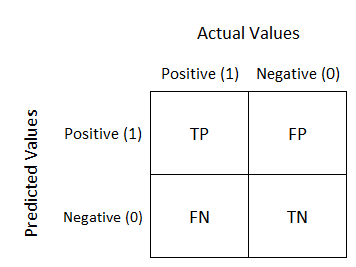
\includegraphics[width=3in]{resources/confusion.png}\\
\end{center}
\end{frame}



\begin{frame}{ROC Curve/ AOC}
\begin{center}
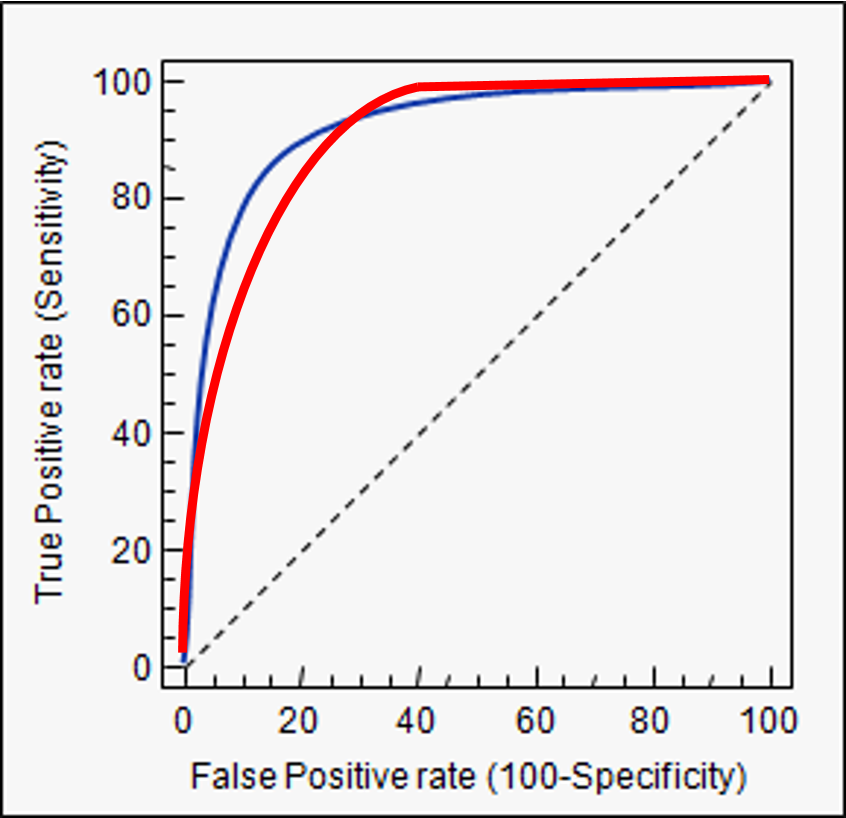
\includegraphics[width=2.5in]{resources/roc_curve.png}\\
\end{center}
\begin{itemize}
\item At each predicted probability calculate both \alert{True Positive Rate} and \alert{False Positive Rate}.
\item AOC is area under the curve
\end{itemize}
\end{frame}


%% LINE


\begin{frame}
\frametitle{Binary Choice: Overview}
Many problems we are interested in look at discrete rather than continuous outcomes.
\begin{itemize}
\item We are familiar with limitations of the linear probability model (LPM)
\begin{itemize}
\item Predictions outside of $[0,1]$
\item Estimates of marginal effects need not be consistent.
\end{itemize}
\item What about the case where $Y$ is binary and a regressor $X$ is endogenous?
\begin{itemize}
\item The usual 2SLS estimator is \alert{NOT consistent}.
\item Or we can ignore the fact that $Y$ is binary...
\item Neither seems like a good option
\end{itemize}
\item Suppose we have panel data on repeated binary choices
\begin{itemize}
\item Adding FE to the probit model produces biased estimates.
\end{itemize}
\end{itemize}
\end{frame}


%\begin{frame}
%\frametitle{Problem \#1: Endogeneity}
%Four possible solutions (maybe there are more?)
%\begin{enumerate}
%\item Close eyes, run the LPM with instruments (Suggested by MHE).
%\item Specify the distribution of errors in first and second stage and do MLE (\texttt{biprobit} in STATA).
%\item Control Function Estimation
%\item `Special Regressor' Methods
%\end{enumerate}
%\end{frame}
%
%\begin{frame}
%\frametitle{Problem \#1: Endogeneity}
%Setup:
%\begin{itemize}
%\item Binary variable $D$: the outcome of interest
%\item $X$ is a vector of observed regressors with coefficient $\beta$ 
%\begin{itemize}
%\item (Can think about $X^e$: endogenous and $X^0$: exogenous).
%\item In an treatment model we might have that $T$ is a binary treatment indicator within $X$
%\end{itemize}
%\item $\epsilon$ is unobserved error. Specifying $f(e)$ can give logit/probit.
%\item Threshold Crossing / Latent Variable Model:
%\begin{eqnarray*}
%D = \mathbf{1}(X \beta + \epsilon \geq 0)
%\end{eqnarray*}
%\item Goal is not usually $\hat{\beta}$ or it's CI, but rather $P(D=1 | X)$ or $\frac{\partial P[D=1 | x] }{\partial X}$ (marginal effects).
%\end{itemize}
%\end{frame}


\begin{frame}
\frametitle{Linear Probability Model}
Consider the LPM with a single continuous regressor
\begin{itemize}
\item LPM prediction departs greatly from CDF long before $[0,1]$ limits.
\item We get probabilities that are too extreme even for $X\hat{\beta}$ ``in bounds''.
\item Some (MHE) argue that though $\hat{Y}$ is flawed, constant marginal effects are still OK.
\end{itemize}
\begin{center}
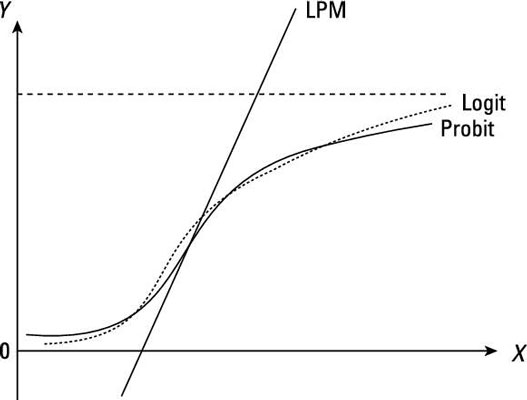
\includegraphics[width=2in]{resources/lpm-probit.jpg}
\end{center}
\end{frame}

\begin{frame}{Some well known textbooks}
(Baby) Wooldrige:
\begin{quote}
``Even with these problems, the linear probability model is useful and often applied in economics. It usually works well for values of the independent variables that are near the averages in the sample.'' (2009, p. 249)
\end{quote}
\begin{itemize}
\item Mentions heteroskedasticity of error (which is binomial given $X$) but does not address the violation of the first LSA.
\end{itemize}
\end{frame}

\begin{frame}{Some well known textbooks}
Angrist and Pischke (MHE) 
\begin{itemize}
\item several examples where marginal effects of probit and LPM are ``indistinguishable''.
\end{itemize}

\begin{quote}
...while a nonlinear model may fit the CEF (conditional expectation function) for LDVs (limited dependent variable models) more closely than a linear model, when it comes to marginal effects, this probably matters little. This optimistic conclusion is not a theorem, but as in the empirical example here, it seems to be fairly robustly true.(2009, p. 107)
\end{quote}
and continue...
\begin{quote}
...extra complexity comes into the inference step as well, since we need standard errors for marginal effects. (ibid.)
\end{quote}
\end{frame}

\begin{frame}
\frametitle{Linear Probability Model}
How does the LPM work?
\begin{eqnarray*}
D = X \beta + \varepsilon
\end{eqnarray*}
\begin{itemize}
\item Estimated $\hat{\beta}$ are the MFX.
\item With exogenous $X$ we have $E[D | X] = Pr[D=1 | X] = X \beta$.
\item If some elements of $X$ (including treatment indicators) are endogenous or mismeasured they will be correlated with $E$.
\item In that case we can do IV via 2SLS or IV-GMM given some instruments $Z$.
\item We need the usual $E[\varepsilon  | X]= 0 $ or $E[\varepsilon | Z] = 0$. \pause
\item An obvious flaw: Given any $\varepsilon | X  $ must equal either $1- X \beta$ or $-X \beta$ which are functions of $X$
\item \alert{Only the trivial binary $X$ with no other regressors satisfies this!}
\end{itemize}
\end{frame}
\begin{frame}
\frametitle{Alarming Example: Lewbel Dong and Yang (2012)}
\begin{itemize}
\item LPM is not just about taste and convenience.
\item Three treated observations, three untreated % \texttt{Treated=1}
\item Assume that $f(\varepsilon) \sim N(0,\sigma^2)$
\begin{eqnarray*}
D = I ( 1 + Treated + R + \varepsilon \geq 0 ) 
\end{eqnarray*}
\item Each individual treatment effect given by:
\begin{eqnarray*}
 I ( 2 + R + \varepsilon \geq 0 ) -  I ( 1 + R + \varepsilon \geq 0 )  =  I ( 0 \leq 1 + R + \varepsilon \leq 1 ) 
\end{eqnarray*}
\item All treatment effects are positive for all $(R,\varepsilon)$.
\item Construct a sample where true effect $=1$ for 5th individual, 0 otherwise. $ATE= \frac{1}{6}$.
\end{itemize}
\end{frame}

\begin{frame}[fragile]
\frametitle{Alarming Example: Lewbel Dong and Yang (2012)}
\tiny
\begin{semiverbatim}
. list
     |     R   Treated   D |
  1. |  -1.8         0   0 | 
  2. |   -.9         0   1 |
  3. |  -.92         0   1 |
  4. |  -2.1         1   0 |
  5. | -1.92         1   1 |
  6. |    10         1   1 |
  \end{semiverbatim}
  \end{frame}
  
\begin{frame}[fragile]
\frametitle{Alarming Example: Lewbel Dong and Yang (2012)}
\tiny
\begin{semiverbatim}
. reg D Treated R, robust

Linear regression                               Number of obs     =          6
                                                F(2, 3)           =       1.02
                                                Prob > F          =     0.4604
                                                R-squared         =     0.1704
                                                Root MSE          =     .60723

------------------------------------------------------------------------------
             |               Robust
           D |      Coef.   Std. Err.      t    P>|t|     [95% Conf. Interval]
-------------+----------------------------------------------------------------
     Treated |  -.1550841   .5844637    -0.27   0.808    -2.015108     1.70494
           R |   .0484638   .0419179     1.16   0.331    -.0849376    .1818651
       _cons |   .7251463   .3676811     1.97   0.143    -.4449791    1.895272
------------------------------------------------------------------------------
. nlcom _b[Treated]/_b[R]
       _nl_1:  _b[Treated]/_b[R]
------------------------------------------------------------------------------
           D |      Coef.   Std. Err.      z    P>|z|     [95% Conf. Interval]
-------------+----------------------------------------------------------------
       _nl_1 |       -3.2   10.23042    -0.31   0.754    -23.25125    16.85125
------------------------------------------------------------------------------
\end{semiverbatim}
\end{frame}

\begin{frame}[fragile]
\frametitle{Alarming Example: Lewbel Dong and Yang (2012)}
\begin{itemize}
\item That went well, except that:
\begin{itemize}
\item we got the wrong sign of $\beta_T$
\item $\beta_1/\beta_2$ was the wrong sign and three times too big.
\end{itemize}
\item this is not because of small sample size or $\beta_1 \approx 0$.
\item As $n \rightarrow \infty$ we can get an arbitrarily precise wrong answer.
\item We don't even get the sign right!
\item This is still in OLS (not much hope for 2SLS).
\end{itemize}
\end{frame}

\begin{frame}[fragile]
\frametitle{Alarming Example: Lewbel Dong and Yang (2012)}
\tiny
\begin{semiverbatim}
. expand 30
(...)
. reg D Treated R, robust

Linear regression                               Number of obs     =        180
                                                F(2, 177)         =      59.93
                                                Prob > F          =     0.0000
                                                R-squared         =     0.1704
                                                Root MSE          =       .433

------------------------------------------------------------------------------
             |               Robust
           D |      Coef.   Std. Err.      t    P>|t|     [95% Conf. Interval]
-------------+----------------------------------------------------------------
     Treated |  -.1550841   .0760907    -2.04   0.043    -.3052458   -.0049224
           R |   .0484638   .0054572     8.88   0.000     .0376941    .0592334
       _cons |   .7251463    .047868    15.15   0.000     .6306808    .8196117
\end{semiverbatim}
\end{frame}



\begin{frame}
\frametitle{Estimating Finite Mixtures}
\begin{itemize}
\item In practice estimating finite mixture models can be tricky.
\item A simple example is the mixture of normals (incomplete data likelihood)
\begin{eqnarray*}
f(x_1,\ldots,x_n | \theta) = \prod_{i=1}^N \sum_{k=1}^K \pi_k f(x_i | \mu_k, \sigma_k)
\end{eqnarray*}
\item We need to find both mixture weights $\pi_k = Pr(z_k)$ and the components $(\mu_k,\sigma_k)$ the weights define a valid probabiltiy measure $\sum_k \pi_k = 1$.
\item Easy problem is \alert{label switching}. Usually it helps to order the components by say decreasing $\pi_1 > \pi_2 > \ldots$ or  $\mu_1 > \mu_2 > \ldots$ 
\item The real problem is that which component you belong to is unobserved. We can add an extra indicator variable $z_{ik} \in \{0,1\}$.
\item We don't care about $z_{ik}$ per-se so they are \alert{nuisance parameters}.
\end{itemize}
\end{frame}

\begin{frame}
\frametitle{Estimating Finite Mixtures}
\begin{itemize}
\item We can write the complete data log-likelihood (as if we observed $z_{ik}$):
\begin{eqnarray*}
\ell(x_1,\ldots,x_n | \theta) = \sum_{i=1}^N  \log \left( \sum_{k=1}^K I[z_i = k]  \pi_k f(x_i \mu_k, \sigma_k) \right)
\end{eqnarray*}
\item We can instead maximized the expected log-likelihood where we take the expectation $E_{z|\theta}$
\begin{eqnarray*}
\alpha_{ik}(\theta) = Pr(z_{ik} =1 | x_i,\theta) = \frac{f_k(x_i,z_k,\mu_k,\sigma_k) \pi_k }{\sum_{m=1}^K f_m(x_i,z_m,\mu_m,\sigma_m) \pi_m}
\end{eqnarray*}
\item Now we have a probability $\hat{\alpha}_{ik}$ that gives us the probability that $i$ came from component $k$. We also compute $\hat{\pi}_k = \frac{1}{N} \sum_{i=1}^N \alpha_{ik}$
\end{itemize}
\end{frame}

\begin{frame}
\frametitle{EM Algorithm}
\begin{itemize}
\item Treat the $\hat{\alpha}_k(\theta^{(q)})$ as data and maximize to find $\mu_k,\sigma_k$ for each $k$
\begin{eqnarray*}
\hat{\theta}^{(q+1)} = \arg \max_{\theta}  \sum_{i=1}^N  \log \left( \sum_{k=1}^K \hat{\alpha}_k(\theta^{(q)}) f(x_i | z_{ik}, \theta ) \right)
\end{eqnarray*}
\item We iterate between updating $\hat{\alpha}_k(\theta^{(q)})$ (E-step) and $\hat{\theta}^{(q+1)}$ (M-step)
\item For the mixture of normals we can compute the M-step very easily:
\begin{eqnarray*}
\mu_k^{(q+1)} &=& \frac{1}{N} \sum_{i=1}^N \hat{\alpha}_k(\theta^{(q)}) x_{i}\\
\sigma_k^{(q+1)} &=& \frac{1}{N} \sum_{i=1}^N \hat{\alpha}_k(\theta^{(q)}) (x_{i} - \overline{x})^2 \\
\end{eqnarray*}
\end{itemize}
\end{frame}

\begin{frame}
\frametitle{EM Algorithm}
\begin{itemize}
\item EM algorithm has the advantage that it avoids complicated integrals in computing the expected log-likelihood over the missing data.
\item For a large set of families it is proven to converge to the MLE
\item That convergence is \alert{monotonic} and \alert{linear}. (Newton's method is quadratic)
\item This means it can be slow, but sometimes $\nabla_{\theta} f (\cdot)$ is really complicated.
\end{itemize}
\end{frame}

\section*{Thanks!}

\end{document}